% Options for packages loaded elsewhere
\PassOptionsToPackage{unicode}{hyperref}
\PassOptionsToPackage{hyphens}{url}
%
\documentclass[
  english,
  man]{apa6}
\usepackage{amsmath,amssymb}
\usepackage{lmodern}
\usepackage{ifxetex,ifluatex}
\ifnum 0\ifxetex 1\fi\ifluatex 1\fi=0 % if pdftex
  \usepackage[T1]{fontenc}
  \usepackage[utf8]{inputenc}
  \usepackage{textcomp} % provide euro and other symbols
\else % if luatex or xetex
  \usepackage{unicode-math}
  \defaultfontfeatures{Scale=MatchLowercase}
  \defaultfontfeatures[\rmfamily]{Ligatures=TeX,Scale=1}
\fi
% Use upquote if available, for straight quotes in verbatim environments
\IfFileExists{upquote.sty}{\usepackage{upquote}}{}
\IfFileExists{microtype.sty}{% use microtype if available
  \usepackage[]{microtype}
  \UseMicrotypeSet[protrusion]{basicmath} % disable protrusion for tt fonts
}{}
\makeatletter
\@ifundefined{KOMAClassName}{% if non-KOMA class
  \IfFileExists{parskip.sty}{%
    \usepackage{parskip}
  }{% else
    \setlength{\parindent}{0pt}
    \setlength{\parskip}{6pt plus 2pt minus 1pt}}
}{% if KOMA class
  \KOMAoptions{parskip=half}}
\makeatother
\usepackage{xcolor}
\IfFileExists{xurl.sty}{\usepackage{xurl}}{} % add URL line breaks if available
\IfFileExists{bookmark.sty}{\usepackage{bookmark}}{\usepackage{hyperref}}
\hypersetup{
  pdftitle={Job Demands-Resources model components through the lens of O*NET classifications},
  pdfauthor={Alicia Stachowski1, Renata Garcia Prieto Palacios Roji2, \& John Kulas2},
  pdflang={en-EN},
  pdfkeywords={keywords},
  hidelinks,
  pdfcreator={LaTeX via pandoc}}
\urlstyle{same} % disable monospaced font for URLs
\usepackage{graphicx}
\makeatletter
\def\maxwidth{\ifdim\Gin@nat@width>\linewidth\linewidth\else\Gin@nat@width\fi}
\def\maxheight{\ifdim\Gin@nat@height>\textheight\textheight\else\Gin@nat@height\fi}
\makeatother
% Scale images if necessary, so that they will not overflow the page
% margins by default, and it is still possible to overwrite the defaults
% using explicit options in \includegraphics[width, height, ...]{}
\setkeys{Gin}{width=\maxwidth,height=\maxheight,keepaspectratio}
% Set default figure placement to htbp
\makeatletter
\def\fps@figure{htbp}
\makeatother
\setlength{\emergencystretch}{3em} % prevent overfull lines
\providecommand{\tightlist}{%
  \setlength{\itemsep}{0pt}\setlength{\parskip}{0pt}}
\setcounter{secnumdepth}{-\maxdimen} % remove section numbering
% Make \paragraph and \subparagraph free-standing
\ifx\paragraph\undefined\else
  \let\oldparagraph\paragraph
  \renewcommand{\paragraph}[1]{\oldparagraph{#1}\mbox{}}
\fi
\ifx\subparagraph\undefined\else
  \let\oldsubparagraph\subparagraph
  \renewcommand{\subparagraph}[1]{\oldsubparagraph{#1}\mbox{}}
\fi
% Manuscript styling
\usepackage{upgreek}
\captionsetup{font=singlespacing,justification=justified}

% Table formatting
\usepackage{longtable}
\usepackage{lscape}
% \usepackage[counterclockwise]{rotating}   % Landscape page setup for large tables
\usepackage{multirow}		% Table styling
\usepackage{tabularx}		% Control Column width
\usepackage[flushleft]{threeparttable}	% Allows for three part tables with a specified notes section
\usepackage{threeparttablex}            % Lets threeparttable work with longtable

% Create new environments so endfloat can handle them
% \newenvironment{ltable}
%   {\begin{landscape}\centering\begin{threeparttable}}
%   {\end{threeparttable}\end{landscape}}
\newenvironment{lltable}{\begin{landscape}\centering\begin{ThreePartTable}}{\end{ThreePartTable}\end{landscape}}

% Enables adjusting longtable caption width to table width
% Solution found at http://golatex.de/longtable-mit-caption-so-breit-wie-die-tabelle-t15767.html
\makeatletter
\newcommand\LastLTentrywidth{1em}
\newlength\longtablewidth
\setlength{\longtablewidth}{1in}
\newcommand{\getlongtablewidth}{\begingroup \ifcsname LT@\roman{LT@tables}\endcsname \global\longtablewidth=0pt \renewcommand{\LT@entry}[2]{\global\advance\longtablewidth by ##2\relax\gdef\LastLTentrywidth{##2}}\@nameuse{LT@\roman{LT@tables}} \fi \endgroup}

% \setlength{\parindent}{0.5in}
% \setlength{\parskip}{0pt plus 0pt minus 0pt}

% \usepackage{etoolbox}
\makeatletter
\patchcmd{\HyOrg@maketitle}
  {\section{\normalfont\normalsize\abstractname}}
  {\section*{\normalfont\normalsize\abstractname}}
  {}{\typeout{Failed to patch abstract.}}
\patchcmd{\HyOrg@maketitle}
  {\section{\protect\normalfont{\@title}}}
  {\section*{\protect\normalfont{\@title}}}
  {}{\typeout{Failed to patch title.}}
\makeatother
\shorttitle{O*NET JD-R}
\keywords{keywords\newline\indent Word count: X}
\DeclareDelayedFloatFlavor{ThreePartTable}{table}
\DeclareDelayedFloatFlavor{lltable}{table}
\DeclareDelayedFloatFlavor*{longtable}{table}
\makeatletter
\renewcommand{\efloat@iwrite}[1]{\immediate\expandafter\protected@write\csname efloat@post#1\endcsname{}}
\makeatother
\usepackage{csquotes}
\ifxetex
  % Load polyglossia as late as possible: uses bidi with RTL langages (e.g. Hebrew, Arabic)
  \usepackage{polyglossia}
  \setmainlanguage[]{english}
\else
  \usepackage[main=english]{babel}
% get rid of language-specific shorthands (see #6817):
\let\LanguageShortHands\languageshorthands
\def\languageshorthands#1{}
\fi
\ifluatex
  \usepackage{selnolig}  % disable illegal ligatures
\fi
\newlength{\cslhangindent}
\setlength{\cslhangindent}{1.5em}
\newlength{\csllabelwidth}
\setlength{\csllabelwidth}{3em}
\newenvironment{CSLReferences}[2] % #1 hanging-ident, #2 entry spacing
 {% don't indent paragraphs
  \setlength{\parindent}{0pt}
  % turn on hanging indent if param 1 is 1
  \ifodd #1 \everypar{\setlength{\hangindent}{\cslhangindent}}\ignorespaces\fi
  % set entry spacing
  \ifnum #2 > 0
  \setlength{\parskip}{#2\baselineskip}
  \fi
 }%
 {}
\usepackage{calc}
\newcommand{\CSLBlock}[1]{#1\hfill\break}
\newcommand{\CSLLeftMargin}[1]{\parbox[t]{\csllabelwidth}{#1}}
\newcommand{\CSLRightInline}[1]{\parbox[t]{\linewidth - \csllabelwidth}{#1}\break}
\newcommand{\CSLIndent}[1]{\hspace{\cslhangindent}#1}

\title{Job Demands-Resources model components through the lens of O*NET classifications}
\author{Alicia Stachowski\textsuperscript{1}, Renata Garcia Prieto Palacios Roji\textsuperscript{2}, \& John Kulas\textsuperscript{2}}
\date{}


\affiliation{\vspace{0.5cm}\textsuperscript{1} University of Wisconsin - Stout\\\textsuperscript{2} Montclair State University}

\abstract{
O*NET work characteristics were rated in terms of relevance, perception as a demand, and perception as a resource. All the results of this current study match the stress-appraisal stuff. Next steps: 1) discuss results within stress-appraisal framework (Lazarus \& Bookman), 2) different literature on challenge and hindrance demands. Job Demands Resources theory that says resources and demands are relatively universal is NOT consistent with these findings. JDR neglects the other 2 literatures. Analytically pull O*Net descriptors that reflect universal demands/resources (e.g., autonomy) and see how much variability there is on those. Maybe forget about cross-walk thing. May actually want to start with this: \url{https://docs.google.com/spreadsheets/d/1ck-72dQ_c-Pl4Xba9W0r__OYo0znlEnV/edit\#gid=1041061499}.

We want to also group items by O*NET categories so there's not so many (that makes ANOVAs more viable)
}



\begin{document}
\maketitle

Given the popularity of the Job Demands-Resources Theory {[}JD-R; Demerouti et al. (2001){]} in exploring questions related to everything from motivation to job design, we aim to explore the intersection between perceptions of job demands and resources, and the broad set of job characteristics provided on O*Net. A series of evaluations were made that used: 1) direct O*Net terminology (both descriptor and response option), and 2) JD-R influenced ratings of demand, challenge, or hindrance. Prior to a description of results, a brief overview of both the JD-R theory, the stress appraisal process, and O*Net is provided.

\hypertarget{the-job-demands-resources-theory}{%
\subsection{The Job demands-Resources Theory}\label{the-job-demands-resources-theory}}

The overarching context for this study is that of the job demands-resources theory, which is an expansion of the well-studied job demands-resources model (Demerouti et al., 2001). One of the major advantages of the job demands-resources theory is that it allows us to model both work environment and job characteristics via job resources and demands. \emph{Resources} include physical, psychological, social, or organizational aspects of the job that may help an employee achieve work goals, reduce job demands, or promote personal growth and development (Demerouti et al., 2001). In contrast, demands include components of a job that require sustained effort, and as such, produce psychological or physiological strain (e.g., high work pressure is frequently cited as a common demand; Demerouti et al. (2001)).
Cognitively, the perception of an element of one's job as a resource or demand activates one of two distinct processes: either health impairment (resulting from demands) or motivation {[}resulting from resources; A. B. Bakker and Demerouti (2014){]}. Pertinent to the current study, demanding job characteristics are frequently often associated with negative outcomes (e.g., A. Bakker et al., 2003), whereas job characteristics deemed resources have been associated with positive organizational outcomes like engagement and motivation (A. B. Bakker et al., 2007).

\hypertarget{objective-vs.-subjective-nature-of-demands-and-resources-the-role-of-appraisal}{%
\subsection{Objective vs.~Subjective Nature of Demands and Resources: The Role of Appraisal}\label{objective-vs.-subjective-nature-of-demands-and-resources-the-role-of-appraisal}}

Searle and Auton (2015) note that the majority of the research on workplace demands is based on apriori classifications of demands. However, the stress experience, or process, described early on by Lazarus and Folkman (1984) is grounded in the assumption that individual appraisals of stressors/demands vary. Their transactional theory or stress and coping states that people continuously appraise stimuli in their environments. An appraisal is the cognitive process whereby meaning is assigned to a stimulus. If a stimulus is appraised as a stressor (threat, challenge, potentially harmful), emotional distress leads to coping of some kind. This action to cope is also associated with another appraisal about the outcome itself and the process continues if the outcomes is not appraised as favorable (Lazarus \& Folkman, 1984). The stress appraisal process suggests that classifying a job characteristic or environmental condition as an objective demand or resource might be in error.

We next consider the (limited) empirical evidence on this topic. First, some relatively recent research suggests that job demands and resources may not be universally appraised or assigned as such. Starting with job demands, Webster et al. (2011), for example, studied workload, role ambiguity, and role conflict demands, and found while that each could be appraised primarily as challenges or hindrances demands, they could also simultaneously be perceived as being both a challenge and hinderance to different degrees. While their study did include resources, it nonetheless points to individual difference on how people perceive stressors at work. Although part of a much larger study on retirement, Sonnega et al. (2018) compared self-reported (subjective) ratings of degree of physical demand, stress, and need for intense concentration from the Health and Retirement Study with objective ratings from O*Net. Correlations physical demand (r = .52), stress (r = .10), and need for intense concentration (r = .14), again suggesting perhaps that our objective ratings of job demands (and resources) may be subject to a greater level of individual difference than assumed. Next considering resources, Schmitz et al. (2019) captured subjective and objective resources in their study of retirement also. Correlations of composite variables for the resources of autonomy (r = .12), recognition of work (r = .07), decision freedom (r = .08), and advancement (r = -.01), while significant, certainly do not reflect high levels of overlap.

We do acknowledge as well, that demands and resources are not necessarily consistent across days, or seasons, for many employees. Downes et al. (2021) meta-analysis addresses this reality in depth, although it is beyond the scope of this project.

\hypertarget{onet-resource}{%
\subsection{O*Net Resource}\label{onet-resource}}

Originally, the Advisory Panel for the Dictionary of Occupational Titles recommended a system that would ``\ldots promote the effective education, training, counseling, and employment of the American workforce. It should accomplish its purpose by providing a database system that identified, defines, classifies, and describes occupations in the economy in an accessible and flexible manner'' (Dictionary of Occupational Titles (US) and Service (1993), p.~6). The result was the now commonly used O*NET. The Occupational Information Network (O*NET; onetonline.org) contains a comprehensive description of occupations (Peterson et al., 2001). This widely accessed database houses hundreds of standardized and occupation-specific descriptors most occupations in the US and these descriptions are continually updated. In fact, there was a call to work with experienced I/O psychologists over the summer to update the content for the \href{https://www.onetonline.org/link/summary/19-3032.00}{Industrial and Organizational Psychologist listing on O*Net}. These data, and the tools provided for free on the website (e.g., Career Exploration Tools, ``My Next Move for Veterans,'' ``My Next Move,'' Toolkit for Business) are frequently used by counselors, students, human resources departments, and researchers to assist potential applicants discover the skills and training they need for the job of their choice, and also employers with information with which to craft job descriptions and help employees determine what skills are needed for promotion.

\hypertarget{current-study}{%
\subsection{Current Study}\label{current-study}}

This paper aims to provide an integration of the theory and practical occupations-focused data on O*Net. Several broad research questions are examined across jobs:

\begin{quote}
\emph{Research Question 1}: Which O*Net job characteristics are consistently rated as job resources?
\end{quote}

\begin{quote}
\emph{Research Question 2}: Which O*Net job characteristics are consistently rated as challenge demands?
\end{quote}

\begin{quote}
\emph{Research Question 3}: Which O*Net job characteristics are consistently rated as hinderance demands?
\end{quote}

The other distinct possibility we expect we may observe is wide variability in the assignment of some job characteristics within the JD-R framework. In fact, a growing body of evidence suggests people may not universally experience job characteristics as challenges or hinderances (e.g., (A. B. Bakker \& Sanz-Vergel, 2013); {[}cavanaugh2000empirical{]}; (Gerich, 2017); (Podsakoff et al., 2007); (Webster et al., 2011)).

Thus, a fourth question of interest explores just that possibility:

\begin{quote}
\emph{Research Question 4}: Does the \textbf{type of work} reported explain variability in the categorization of work characteristics into challenges, hindrances, and resources?
\end{quote}

\hypertarget{participants}{%
\subsection{Participants}\label{participants}}

Of the 785 Prolific panel individuals who initially accessed the survey link, 112 indicated that they were not interested, had more than 200 missing responses, or had 20 or more identical consecutive sequential responses (\textbf{R-careless?}). Applying a further screen regarding attention checks (there were four attention checks embedded throughout, asking respondents to indicate a specific answer) resulted in the retention of 568 respondents who constitute the current SIOP sample. 13.57\% had been in their referent job less than 6 months, 19.20\% between 6 months and a year, 49.12\% between one and five years, 13.27\% between 5 and 10 years, and 4.87\% more than 10 years.

Ages ranged from 18 to 65 with an average of 28.18 years old (SD = 7.53). The survey offered a free-field gender identity category, although the sample predominantly self-identified as female (52.58\%) or male (46.83\%).

\hypertarget{materials}{%
\subsection{Materials}\label{materials}}

Each free-field job title was placed into one of 14 possible O*NET job families classifications. 60 of these ratings were performed by all 3 author raters, with a resulting Kappa of 0.53 (Landis \& Koch, 1977).

\hypertarget{characteristics-demands-and-resources}{%
\subsubsection{Characteristics, Demands, and Resources}\label{characteristics-demands-and-resources}}

We used 98 statements taken from O*NET \href{https://www.O*NETonline.org/find/descriptor/result/4.A.1.b.3}{``activity'' and ``context'' classifications}. We retained 41 ``work activity'' classifications which O*NET groups into categories of ``Information Input'' (5 statements), ``Interacting with Others'' (17 statements), ``Mental Processes'' (10 statements) and ``Work Output'' (9 statements). 57 ``work context'' statements grouped into ``Interpersonal Relationships'' (14 statements), ``Physical Work Conditions'' (30 statements), and ``Structural Job Characteristics'' (13 statements).

These ``descriptors'' often have unique response categories (\href{https://www.O*NETonline.org/find/descriptor/result/4.C.1.c.2}{see here for example}). We retained the O*NET wording to capture characteristics of relevance for each respondent. Subsequent to these self evaluations, each respondent who agreed that the element had \emph{at least some relevance} to their job was also asked to rate that element in terms of, 1) \ldots this aspect of your job is a resource that can be functional in achieving work goals, reduce job demands, or stimulate personal growth/development, 2) \ldots this aspect of your job is a challenge that can promote mastery, personal growth, or future gains, and 3) \ldots this aspect of your job is a hinderance that can inhibit personal growth, learning, and work goal attainment.

\hypertarget{results}{%
\section{Results}\label{results}}

\hypertarget{low-variability-demands-and-resources}{%
\subsection{Low Variability Demands and Resources}\label{low-variability-demands-and-resources}}

The below graphs present the resources, challenges, and hindrances that are \emph{largely agreed on} as indexed by (relatively) low standard deviations.

\begin{quote}
Note. The ``zero'' standard deviations are likely one person, \emph{n}'s should also go on these graphs if they're retained.
\end{quote}

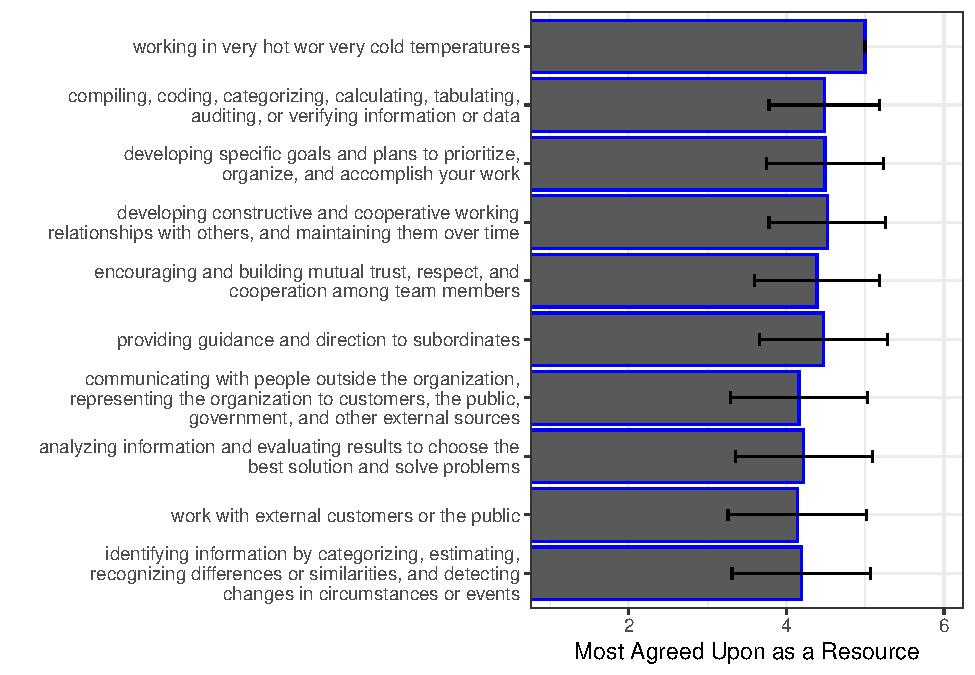
\includegraphics{Submission_files/figure-latex/resourceslowsd-1.pdf}

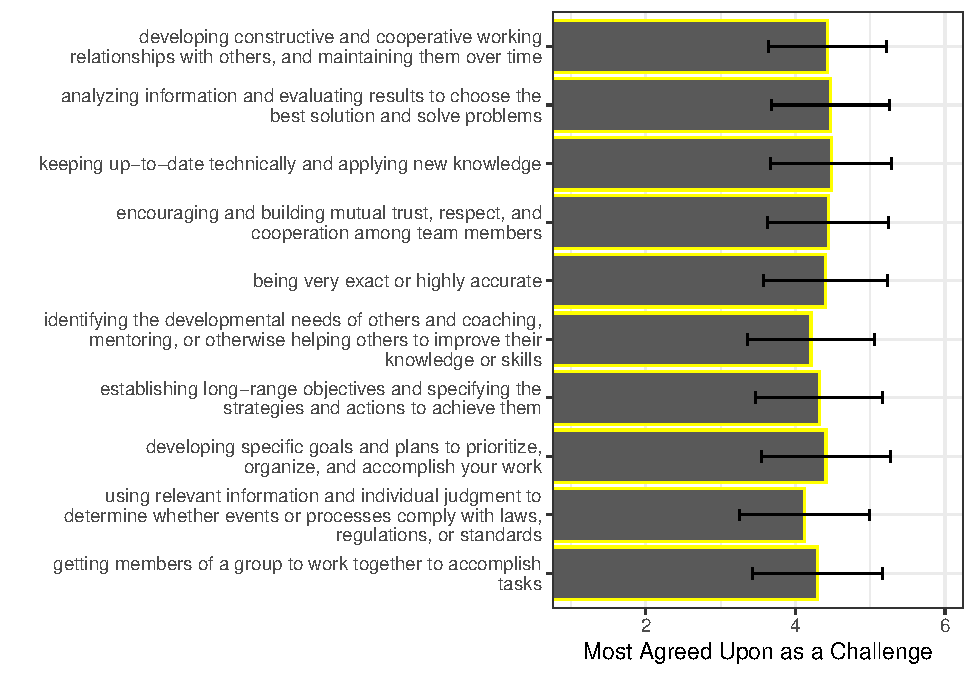
\includegraphics{Submission_files/figure-latex/challengesagree-1.pdf}

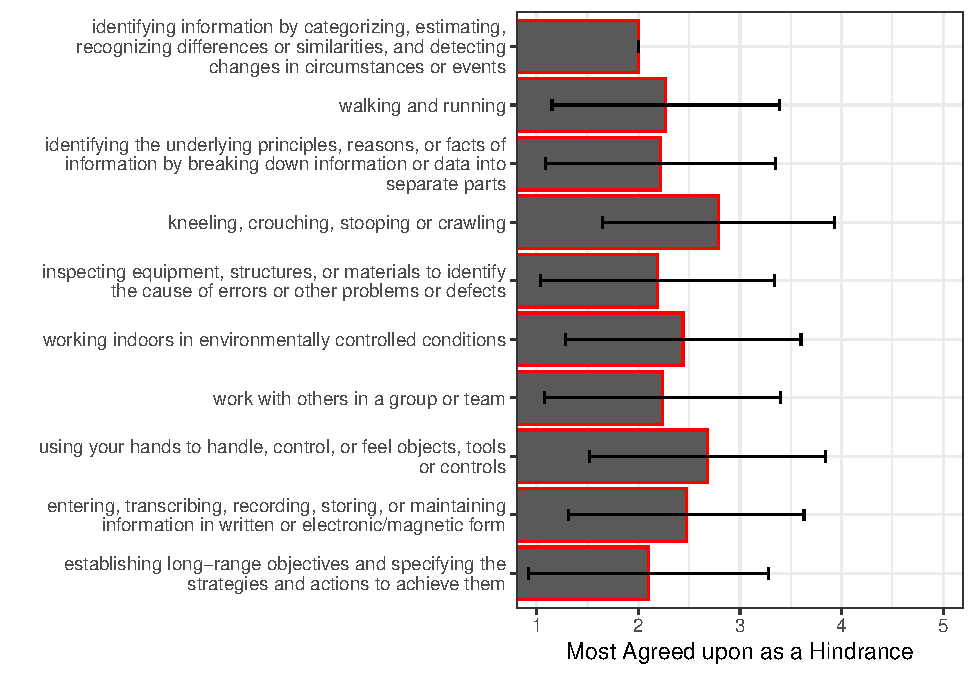
\includegraphics{Submission_files/figure-latex/hindrancesagree-1.pdf}

As can be seen by the graphs, there is considerable disagreement regarding the degree to which job elements are considered \emph{hindrances}, with the 10 elements showing the greatest agreement still ranging in standard deviations from 0 to 1.18. What is widely seen as a resource and challenge tends to be more universally agreed upon (range of lowest 10 resource standard deviations is 0 to 0.88 and the range of lowest 10 challenge standard deviations is 0 to 0.87.

\hypertarget{high-variability-demands-and-resources}{%
\subsection{High Variability Demands and Resources}\label{high-variability-demands-and-resources}}

The below graphs present the resources, challenges, and hindrances that are \emph{largely disagreed on} as indexed by (relatively) high standard deviations (these are the 10 characteristics with the greatest variability in rating).

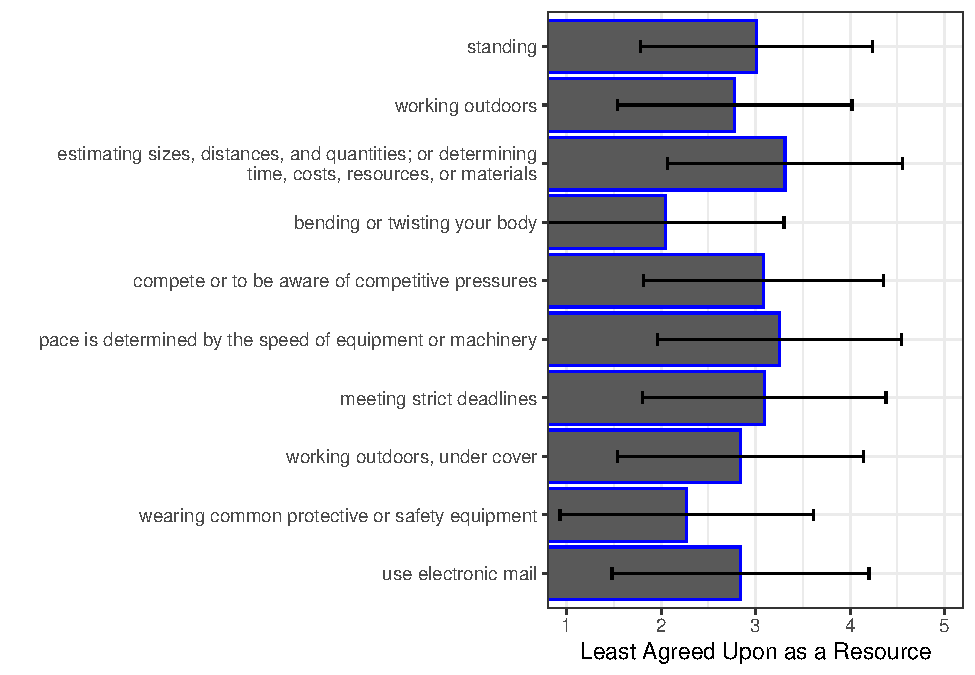
\includegraphics{Submission_files/figure-latex/resourceshisd-1.pdf}

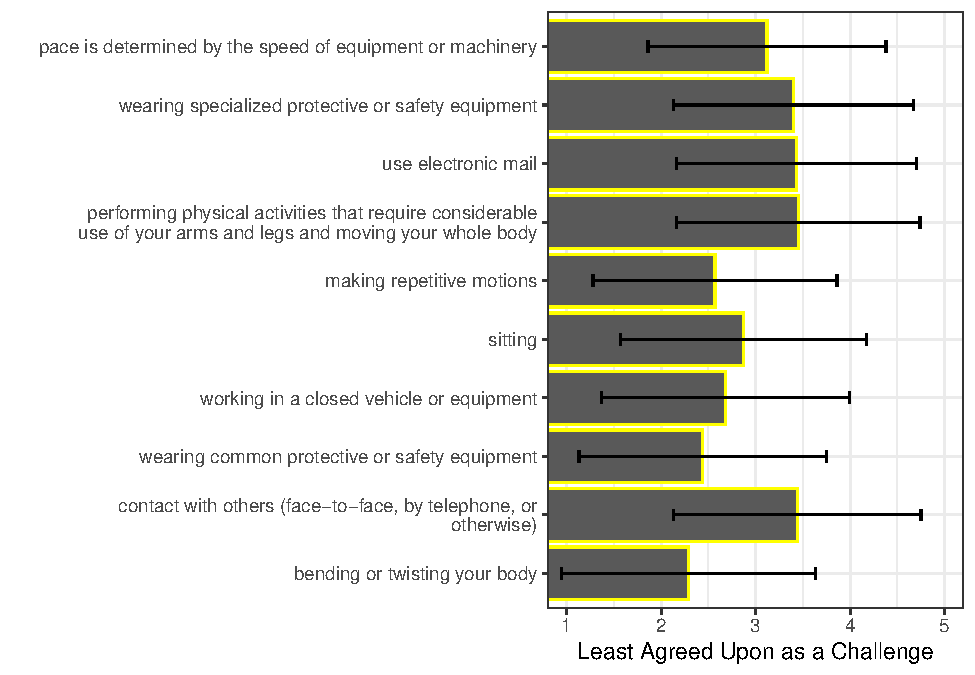
\includegraphics{Submission_files/figure-latex/challengeshighsd-1.pdf}

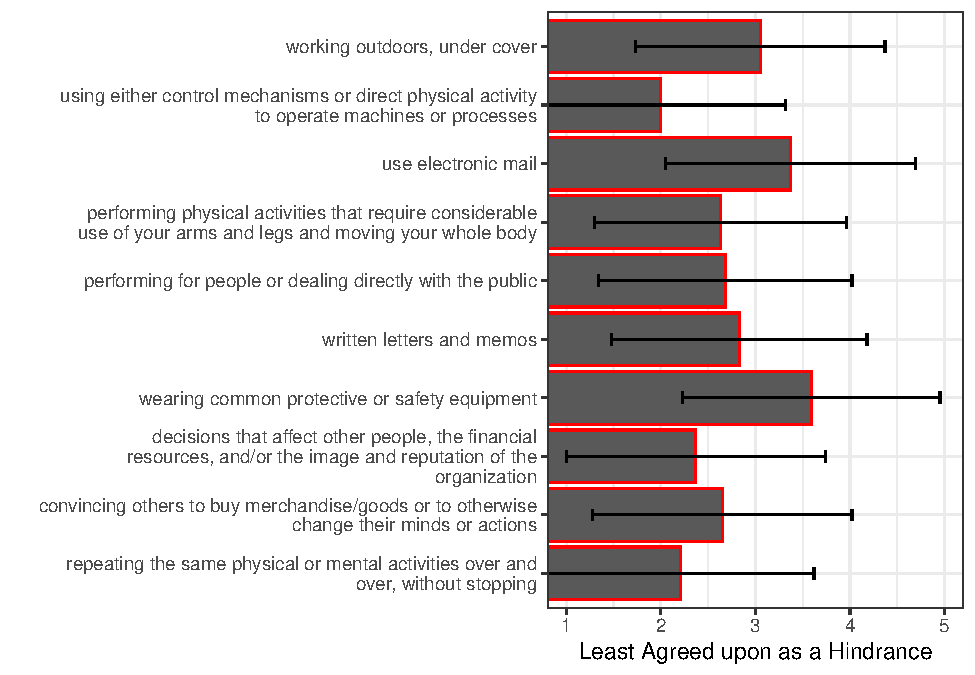
\includegraphics{Submission_files/figure-latex/hindranceshighsd-1.pdf}

\newpage

\hypertarget{references}{%
\section{References}\label{references}}

\begingroup
\setlength{\parindent}{-0.5in}
\setlength{\leftskip}{0.5in}

\hypertarget{refs}{}
\begin{CSLReferences}{1}{0}
\leavevmode\hypertarget{ref-bakker2014job}{}%
Bakker, A. B., \& Demerouti, E. (2014). Job demands--resources theory. \emph{Wellbeing: A Complete Reference Guide}, 1--28.

\leavevmode\hypertarget{ref-bakker2007job}{}%
Bakker, A. B., Hakanen, J. J., Demerouti, E., \& Xanthopoulou, D. (2007). Job resources boost work engagement, particularly when job demands are high. \emph{Journal of Educational Psychology}, \emph{99}(2), 274.

\leavevmode\hypertarget{ref-bakker2013weekly}{}%
Bakker, A. B., \& Sanz-Vergel, A. I. (2013). Weekly work engagement and flourishing: The role of hindrance and challenge job demands. \emph{Journal of Vocational Behavior}, \emph{83}(3), 397--409.

\leavevmode\hypertarget{ref-bakker2003dual}{}%
Bakker, A., Demerouti, E., \& Schaufeli, W. (2003). Dual processes at work in a call centre: An application of the job demands--resources model. \emph{European Journal of Work and Organizational Psychology}, \emph{12}(4), 393--417.

\leavevmode\hypertarget{ref-demerouti2001job}{}%
Demerouti, E., Bakker, A. B., Nachreiner, F., \& Schaufeli, W. B. (2001). The job demands-resources model of burnout. \emph{Journal of Applied Psychology}, \emph{86}(3), 499.

\leavevmode\hypertarget{ref-advisory1993new}{}%
Dictionary of Occupational Titles (US), A. P. for the, \& Service, U. S. E. (1993). \emph{The new DOT: A database of occupational titles for the twenty-first century}. US Department of Labor, Employment; Training Administration, US~\ldots.

\leavevmode\hypertarget{ref-downes2021incorporating}{}%
Downes, P. E., Reeves, C. J., McCormick, B. W., Boswell, W. R., \& Butts, M. M. (2021). Incorporating job demand variability into job demands theory: A meta-analysis. \emph{Journal of Management}, \emph{47}(6), 1630--1656.

\leavevmode\hypertarget{ref-gerich2017relevance}{}%
Gerich, J. (2017). The relevance of challenge and hindrance appraisals of working conditions for employees' health. \emph{International Journal of Stress Management}, \emph{24}(3), 270.

\leavevmode\hypertarget{ref-landis1977measurement}{}%
Landis, J. R., \& Koch, G. G. (1977). The measurement of observer agreement for categorical data. \emph{Biometrics}, 159--174.

\leavevmode\hypertarget{ref-lazarus1984stress}{}%
Lazarus, R. S., \& Folkman, S. (1984). \emph{Stress, appraisal, and coping}. Springer publishing company.

\leavevmode\hypertarget{ref-peterson2001understanding}{}%
Peterson, N. G., Mumford, M. D., Borman, W. C., Jeanneret, P. R., Fleishman, E. A., Levin, K. Y., Campion, M. A., Mayfield, M. S., Morgeson, F. P., Pearlman, K., \& others. (2001). Understanding work using the occupational information network (o* NET): Implications for practice and research. \emph{Personnel Psychology}, \emph{54}(2), 451--492.

\leavevmode\hypertarget{ref-podsakoff2007differential}{}%
Podsakoff, N. P., LePine, J. A., \& LePine, M. A. (2007). Differential challenge stressor-hindrance stressor relationships with job attitudes, turnover intentions, turnover, and withdrawal behavior: A meta-analysis. \emph{Journal of Applied Psychology}, \emph{92}(2), 438.

\leavevmode\hypertarget{ref-schmitz_interpreting_2019}{}%
Schmitz, L. L., McCluney, C. L., Sonnega, A., \& Hicken, M. T. (2019). Interpreting {Subjective} and {Objective} {Measures} of {Job} {Resources}: {The} {Importance} of {Sociodemographic} {Context}. \emph{International Journal of Environmental Research and Public Health}, \emph{16}(17), 3058. \url{https://doi.org/10.3390/ijerph16173058}

\leavevmode\hypertarget{ref-searle2015merits}{}%
Searle, B. J., \& Auton, J. C. (2015). The merits of measuring challenge and hindrance appraisals. \emph{Anxiety, Stress, \& Coping}, \emph{28}(2), 121--143.

\leavevmode\hypertarget{ref-sonnega_comparison_2018}{}%
Sonnega, A., Helppie-McFall, B., Hudomiet, P., Willis, R. J., \& Fisher, G. G. (2018). A {Comparison} of {Subjective} and {Objective} {Job} {Demands} and {Fit} {With} {Personal} {Resources} as {Predictors} of {Retirement} {Timing} in a {National} {U}.{S}. {Sample}. \emph{Work, Aging and Retirement}, \emph{4}(1), 37--51. \url{https://doi.org/10.1093/workar/wax016}

\leavevmode\hypertarget{ref-webster2011extending}{}%
Webster, J. R., Beehr, T. A., \& Love, K. (2011). Extending the challenge-hindrance model of occupational stress: The role of appraisal. \emph{Journal of Vocational Behavior}, \emph{79}(2), 505--516.

\end{CSLReferences}

\endgroup


\end{document}
